\section{definition10}
\begin{definition}
\end{definition}


Suppose we have the following diagram :

\begin{figure}[H] % Optional: [h] means here, [t] for top, [b] for bottom, [p] for page of floats
    \centering
    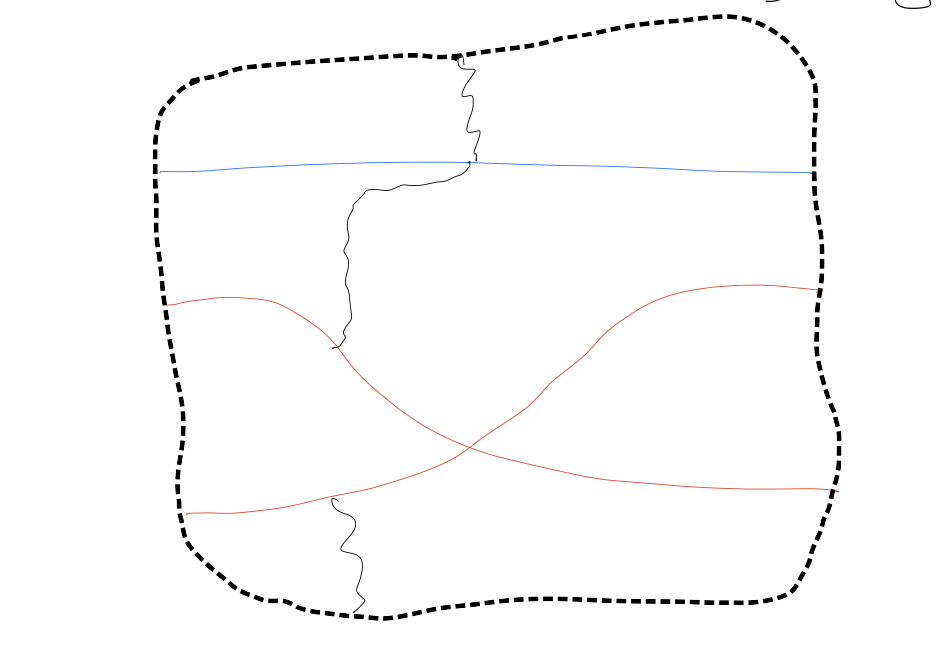
\includegraphics[width=\linewidth]{diagrams/definition10/1.png} % Adjust the width as needed
    \caption{Your caption here}
    \label{fig:your-label}
\end{figure}

We define MOVE \RN{10} as follows :

(Step1) Apply MOVE \RN{1} to the region inside of the purple circle :

\begin{figure}[H] % Optional: [h] means here, [t] for top, [b] for bottom, [p] for page of floats
    \centering
    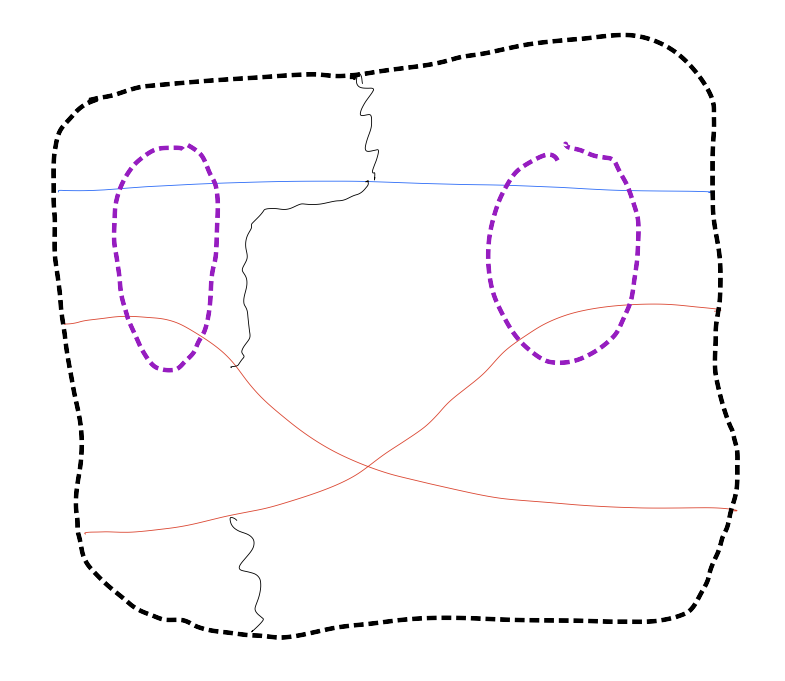
\includegraphics[width=\linewidth]{diagrams/definition10/2.png} % Adjust the width as needed
    \caption{Your caption here}
    \label{fig:your-label}
\end{figure}

we get :

\begin{figure}[H] % Optional: [h] means here, [t] for top, [b] for bottom, [p] for page of floats
    \centering
    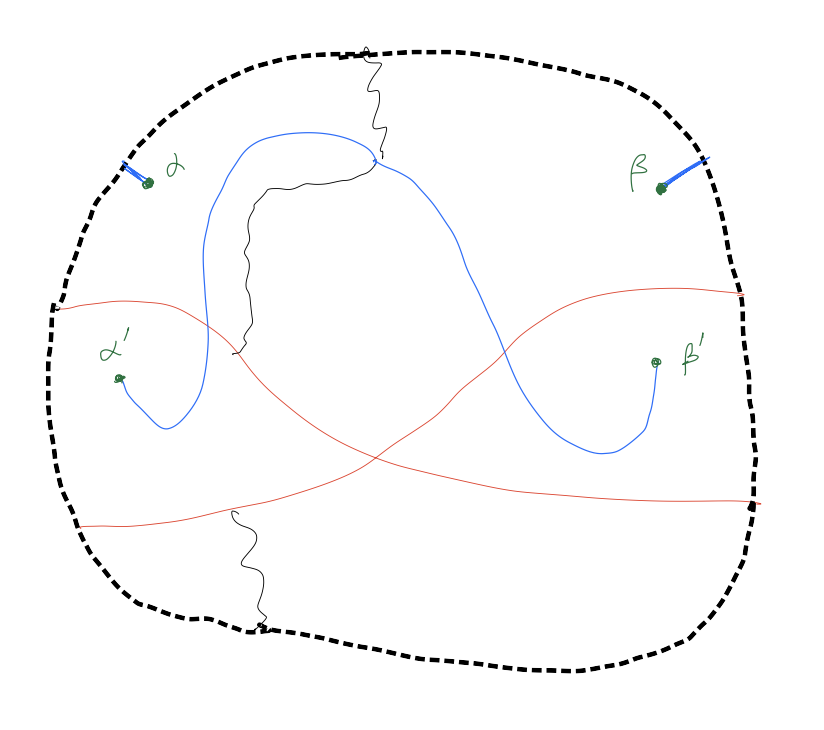
\includegraphics[width=\linewidth]{diagrams/definition10/3.png} % Adjust the width as needed
    \caption{Your caption here}
    \label{fig:your-label}
\end{figure}

(Step2) Apply MOVE \RN{1} to the region inside the purple circle :

\begin{figure}[H] % Optional: [h] means here, [t] for top, [b] for bottom, [p] for page of floats
    \centering
    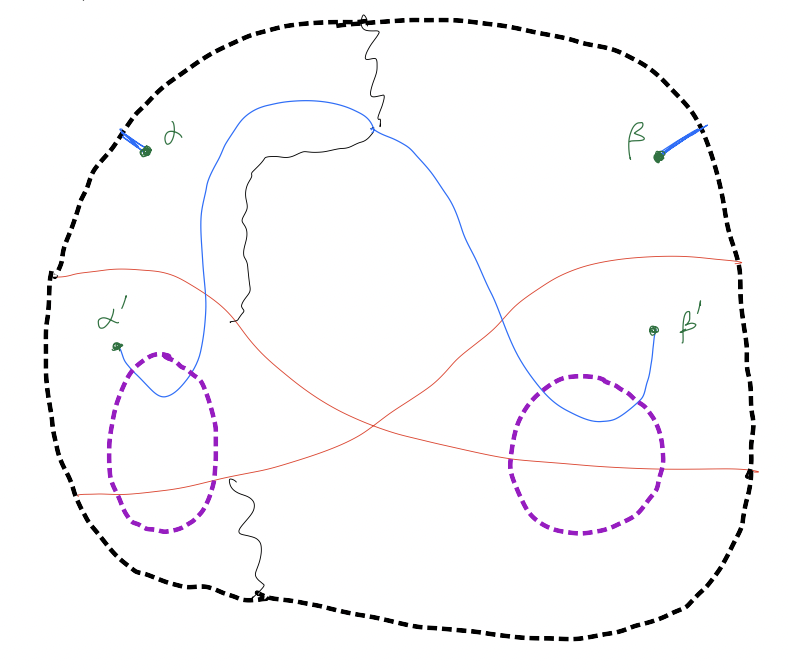
\includegraphics[width=\linewidth]{diagrams/definition10/4.png} % Adjust the width as needed
    \caption{Your caption here}
    \label{fig:your-label}
\end{figure}

we get :

\begin{figure}[H] % Optional: [h] means here, [t] for top, [b] for bottom, [p] for page of floats
    \centering
    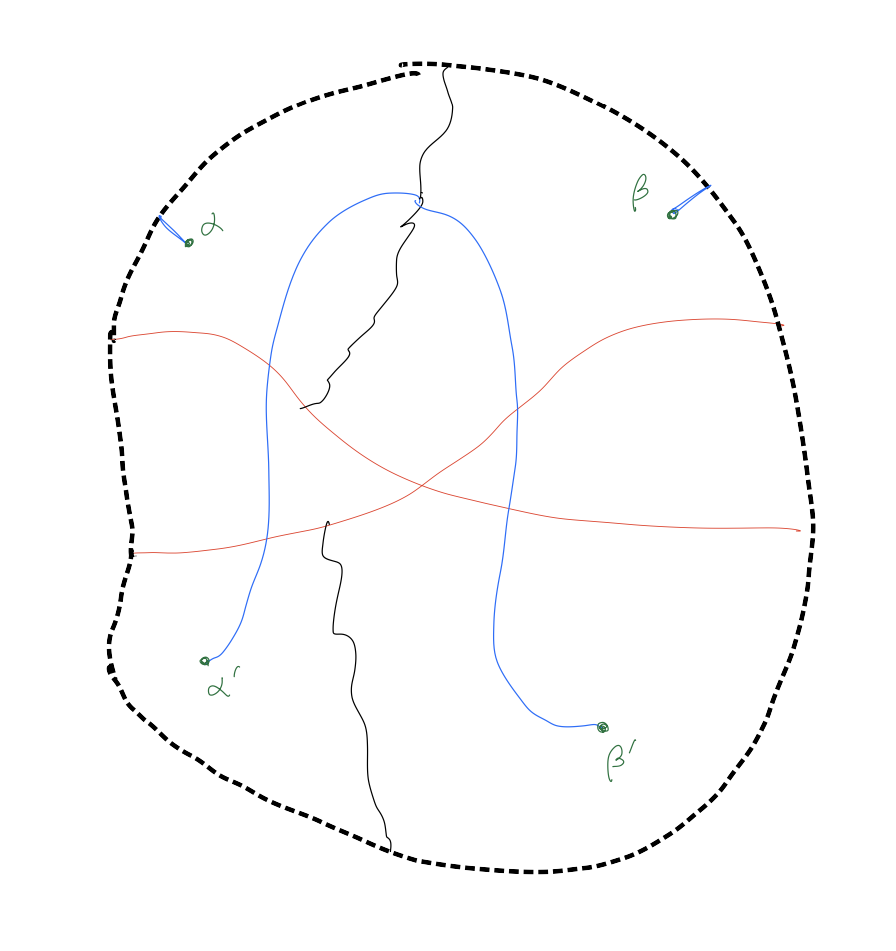
\includegraphics[width=\linewidth]{diagrams/definition10/5.png} % Adjust the width as needed
    \caption{Your caption here}
    \label{fig:your-label}
\end{figure}

(Step3) Apply MOVE \RN{4} to the region inside the purple circle :

\begin{figure}[H] % Optional: [h] means here, [t] for top, [b] for bottom, [p] for page of floats
    \centering
    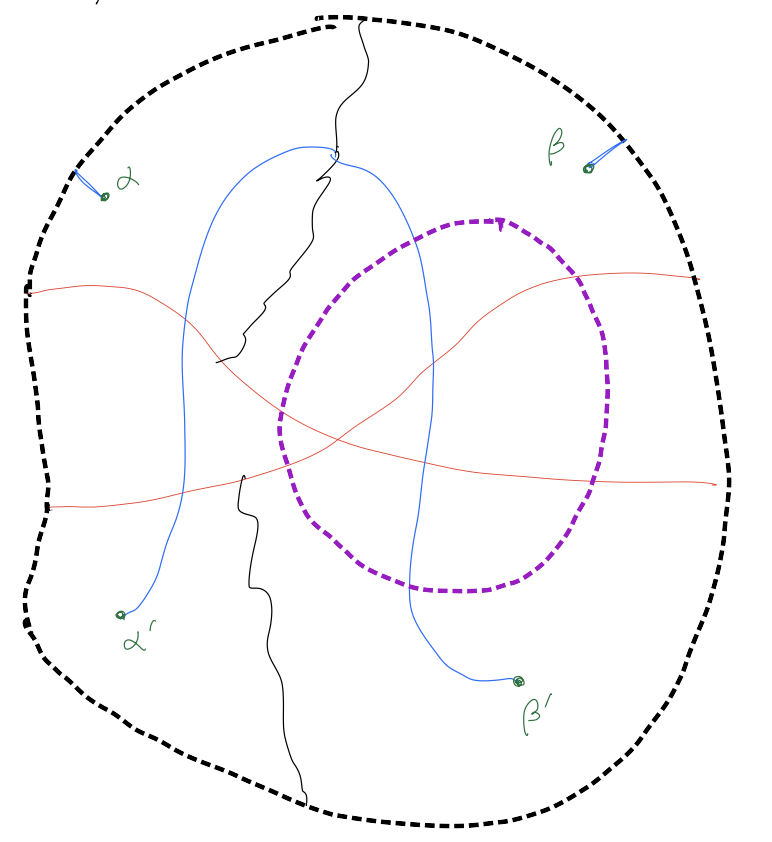
\includegraphics[width=\linewidth]{diagrams/definition10/6.png} % Adjust the width as needed
    \caption{Your caption here}
    \label{fig:your-label}
\end{figure}

we get :

\begin{figure}[H] % Optional: [h] means here, [t] for top, [b] for bottom, [p] for page of floats
    \centering
    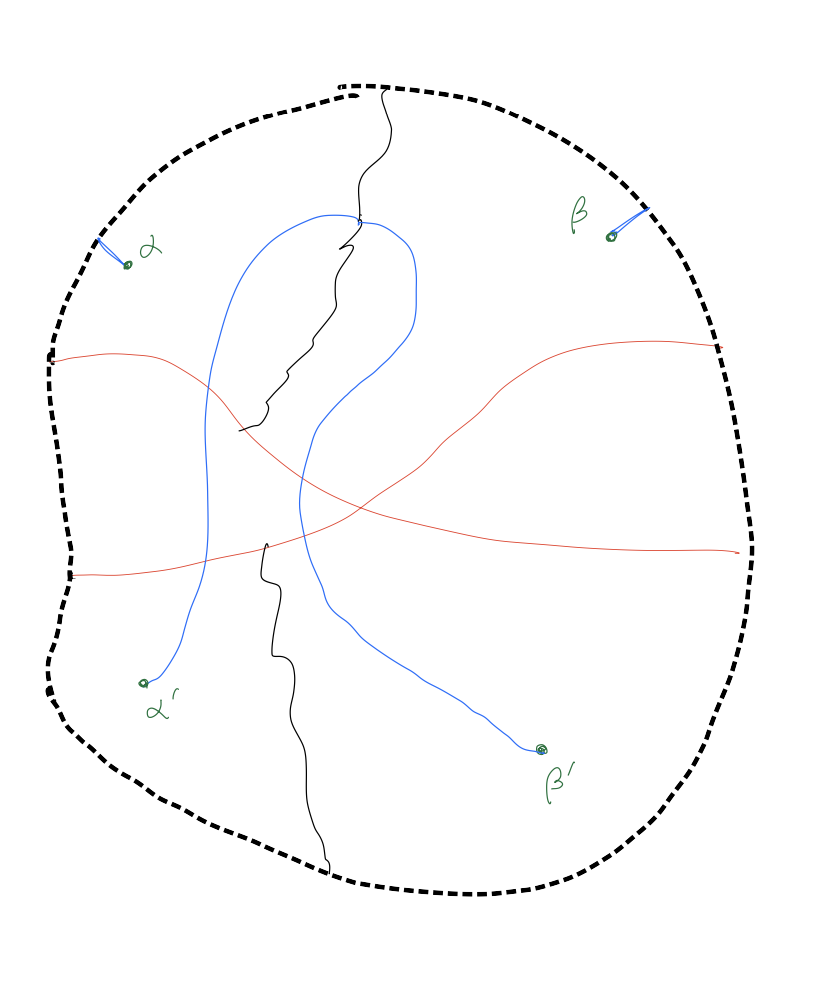
\includegraphics[width=\linewidth]{diagrams/definition10/7.png} % Adjust the width as needed
    \caption{Your caption here}
    \label{fig:your-label}
\end{figure}

(Step4) Apply MOVE \RN{3} to the region inside the purple circle :

\begin{figure}[H] % Optional: [h] means here, [t] for top, [b] for bottom, [p] for page of floats
    \centering
    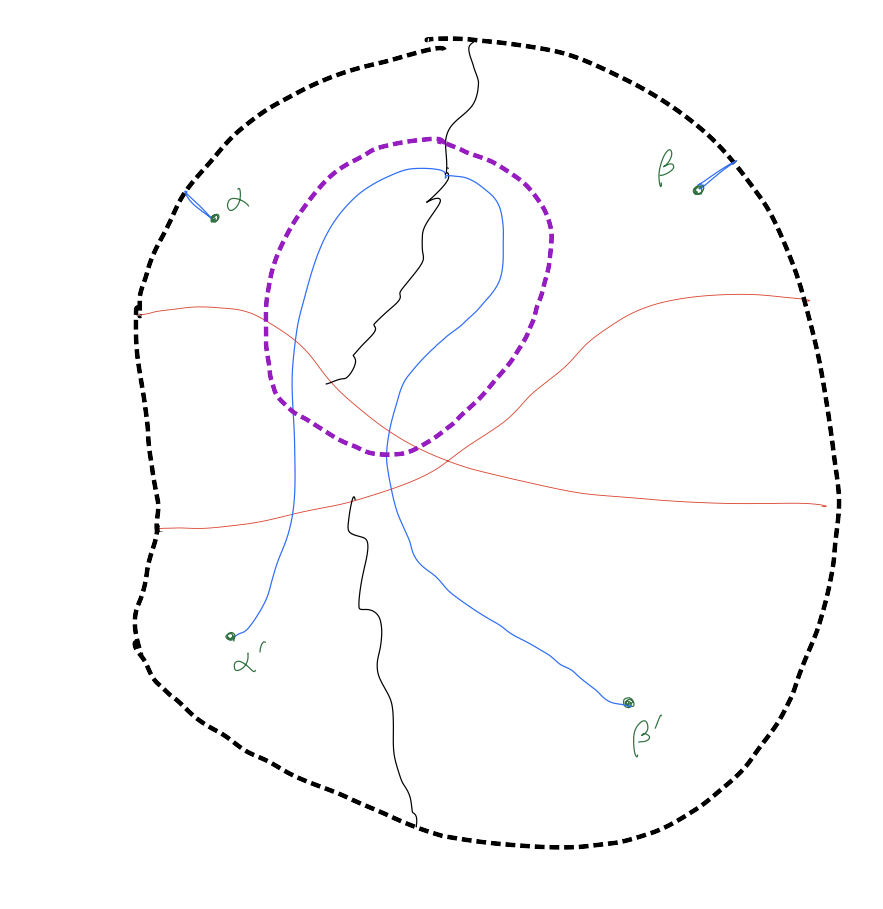
\includegraphics[width=\linewidth]{diagrams/definition10/8.png} % Adjust the width as needed
    \caption{Your caption here}
    \label{fig:your-label}
\end{figure}

we get :

\begin{figure}[H] % Optional: [h] means here, [t] for top, [b] for bottom, [p] for page of floats
    \centering
    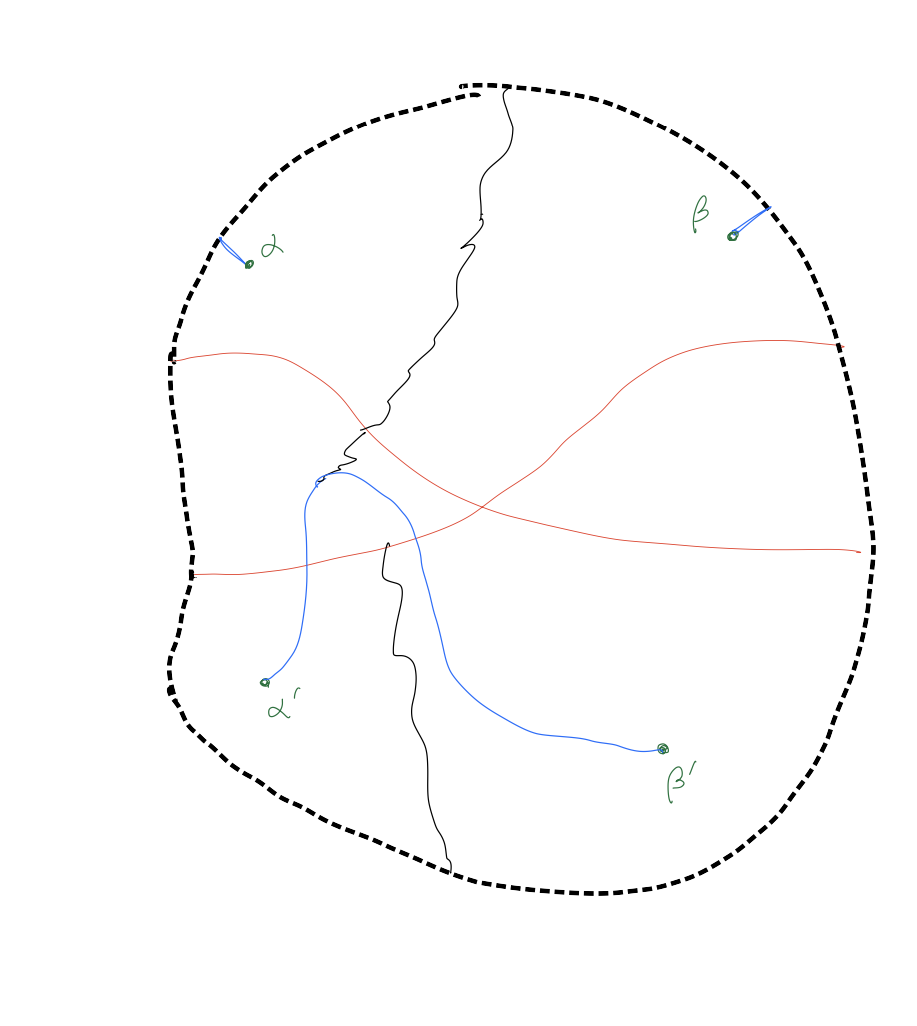
\includegraphics[width=\linewidth]{diagrams/definition10/9.png} % Adjust the width as needed
    \caption{Your caption here}
    \label{fig:your-label}
\end{figure}

(Step5) Apply MOVE \RN{5} to the region inside the purple circle :

\begin{figure}[H] % Optional: [h] means here, [t] for top, [b] for bottom, [p] for page of floats
    \centering
    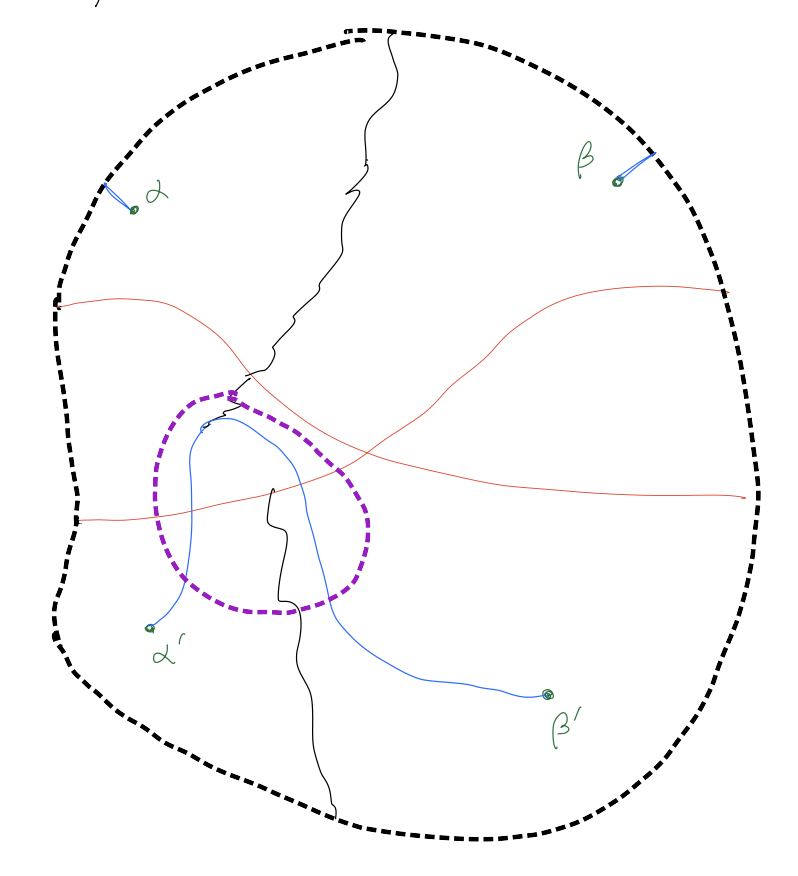
\includegraphics[width=\linewidth]{diagrams/definition10/10.png} % Adjust the width as needed
    \caption{Your caption here}
    \label{fig:your-label}
\end{figure}

we get the final diagram :

\begin{figure}[H] % Optional: [h] means here, [t] for top, [b] for bottom, [p] for page of floats
    \centering
    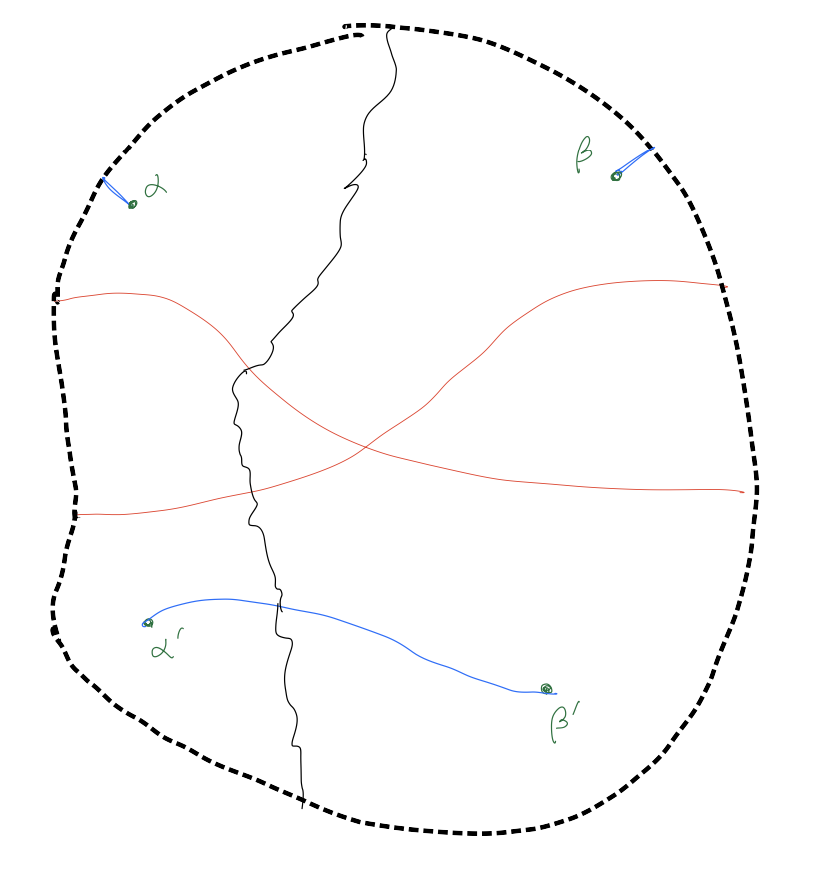
\includegraphics[width=\linewidth]{diagrams/definition10/11.png} % Adjust the width as needed
    \caption{Your caption here}
    \label{fig:your-label}
\end{figure}